\section{Modification of the Christensen-Burley profile to better fit Monte
Carlo references}

The original formulation of the Christensen-Burley BSSRDF, first described in the
\cite{Burley:disney_siggraph15} and enhanced in \cite{Christensen:2015:ARP:2775280.2792555}, is
based on the fitting of the empirically chosen function to the Monte Carlo reference SSS renderings.
That function contains the sum of two exponentials, $1/r$ factor and the normalization coefficient
\ref{eq:burley}.
\[ R_d(r) = As\dfrac{e^{-sr}+e^{-sr/3}}{8\pi r} \]

The exact form of scaling factor $s$ is also determined empirically. For searchlight
configuration has a form:
\begin{equation}
\label{eq:cb_scaling}
s=1.85-A + 7|A - 0.8|^3
\end{equation}

The results of my implementation of the original Christensen-Burley profile are shown as an example
of rendered sample at the figure \ref{fig:burley_searchlight_renders}. The corresponding plots are
provided at figure \ref{fig:burley_fitting}

\begin{figure}[h]
    \centering
    
\includegraphics[width=\textwidth]{imgs/renders/cb_montecarlo_slice}
    
\includegraphics[width=\textwidth]{imgs/renders/cb_modified_slice}
    
\includegraphics[width=\textwidth]{imgs/renders/cb_original_slice}
    \caption{Region of rendered image of Searchlight configuration. From top to bottom: Monte Carlo
    reference, modified Christensen-Burley, original Christensen-Burley}
    \label{fig:burley_searchlight_renders}
\end{figure}

\begin{figure}[h]
    \centering
    \begin{subfigure}{\textwidth}
        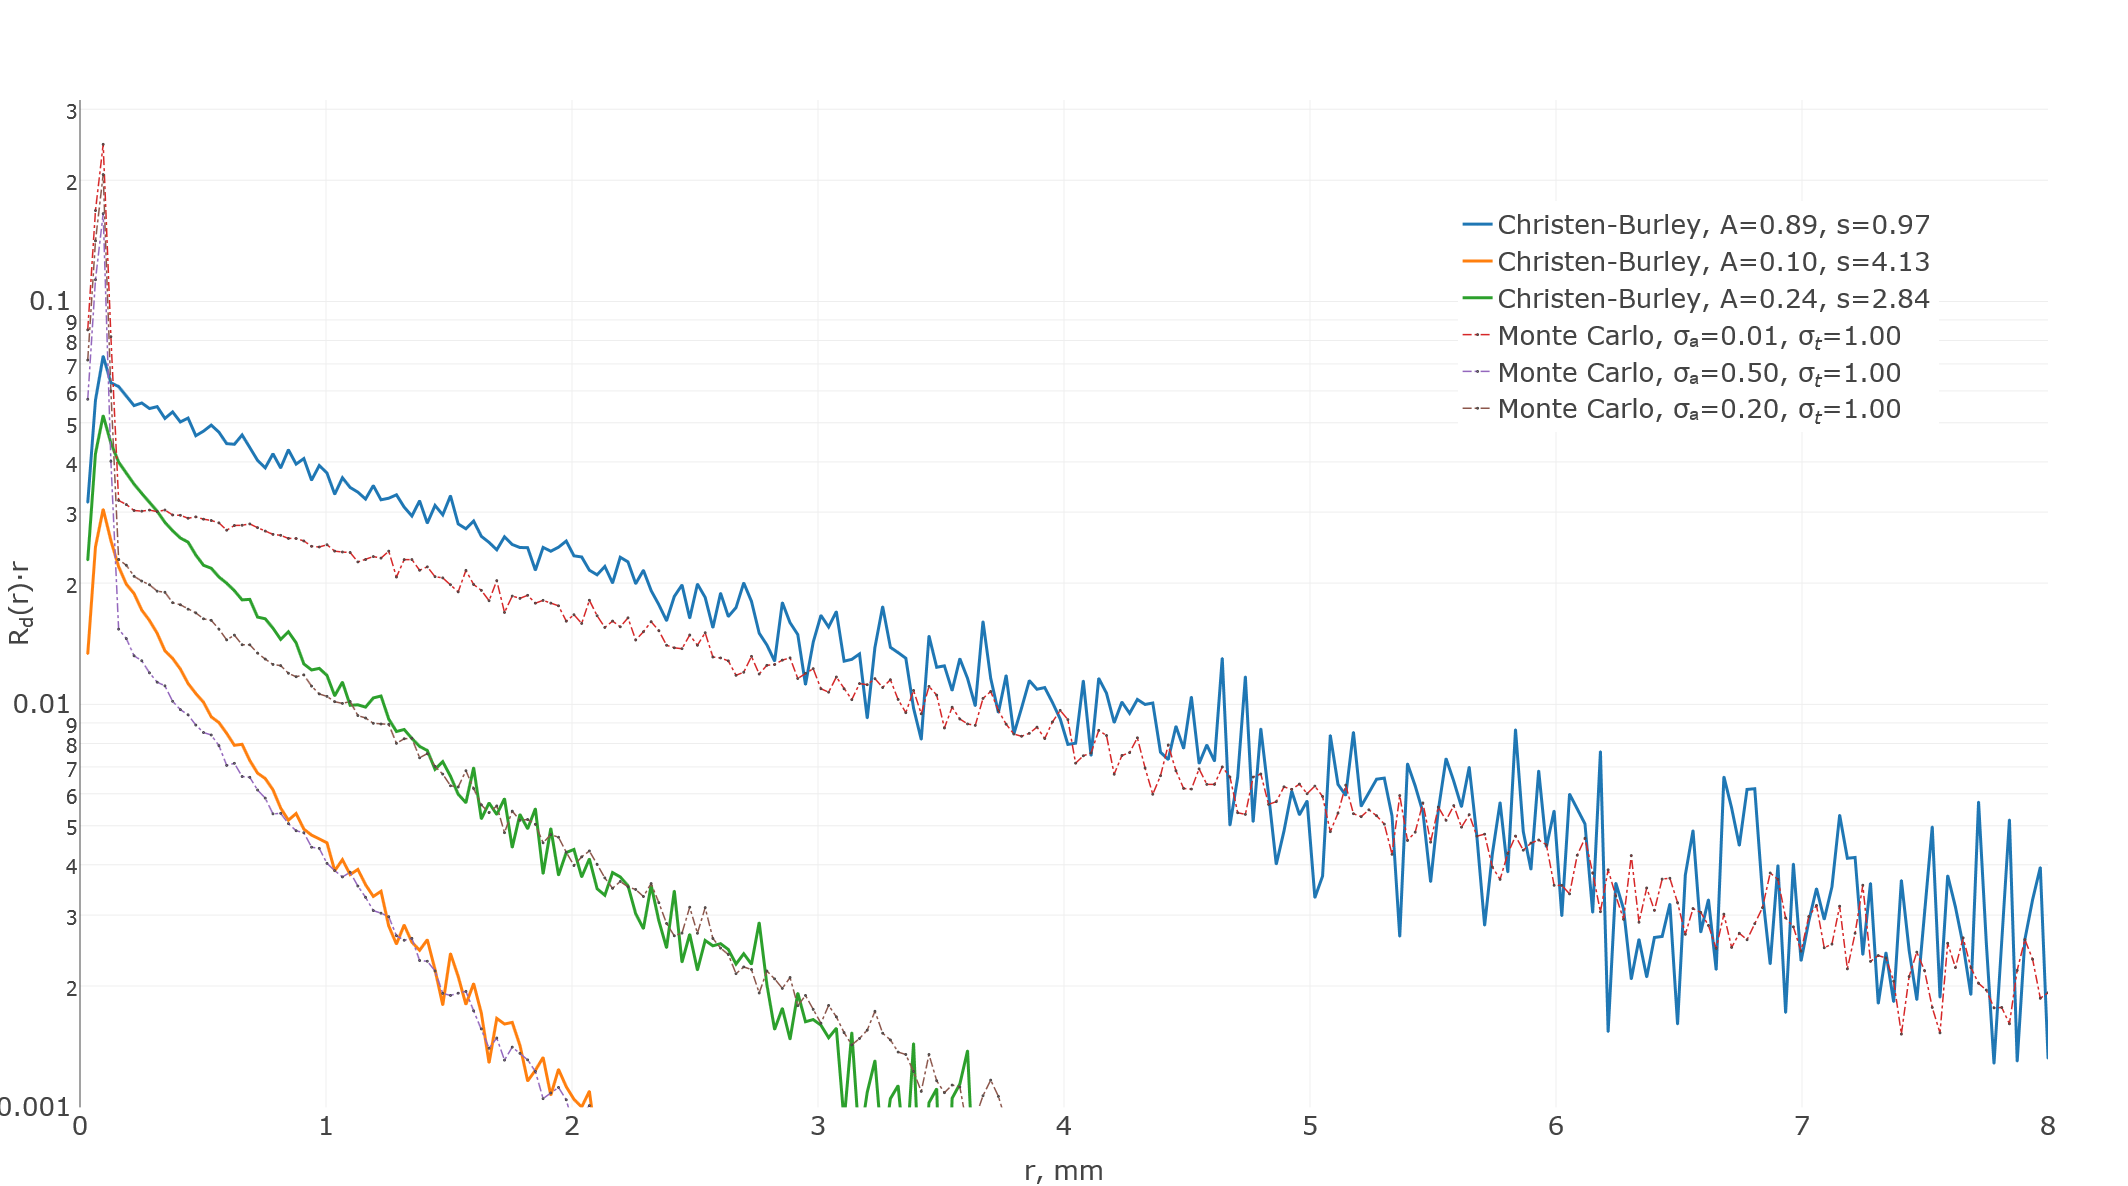
\includegraphics[width=\textwidth]{imgs/plots/cb_original_fitting}
        \caption{Original Christensen-Burley over Monte Carlo reference}
    \end{subfigure}
    \begin{subfigure}{\textwidth}
        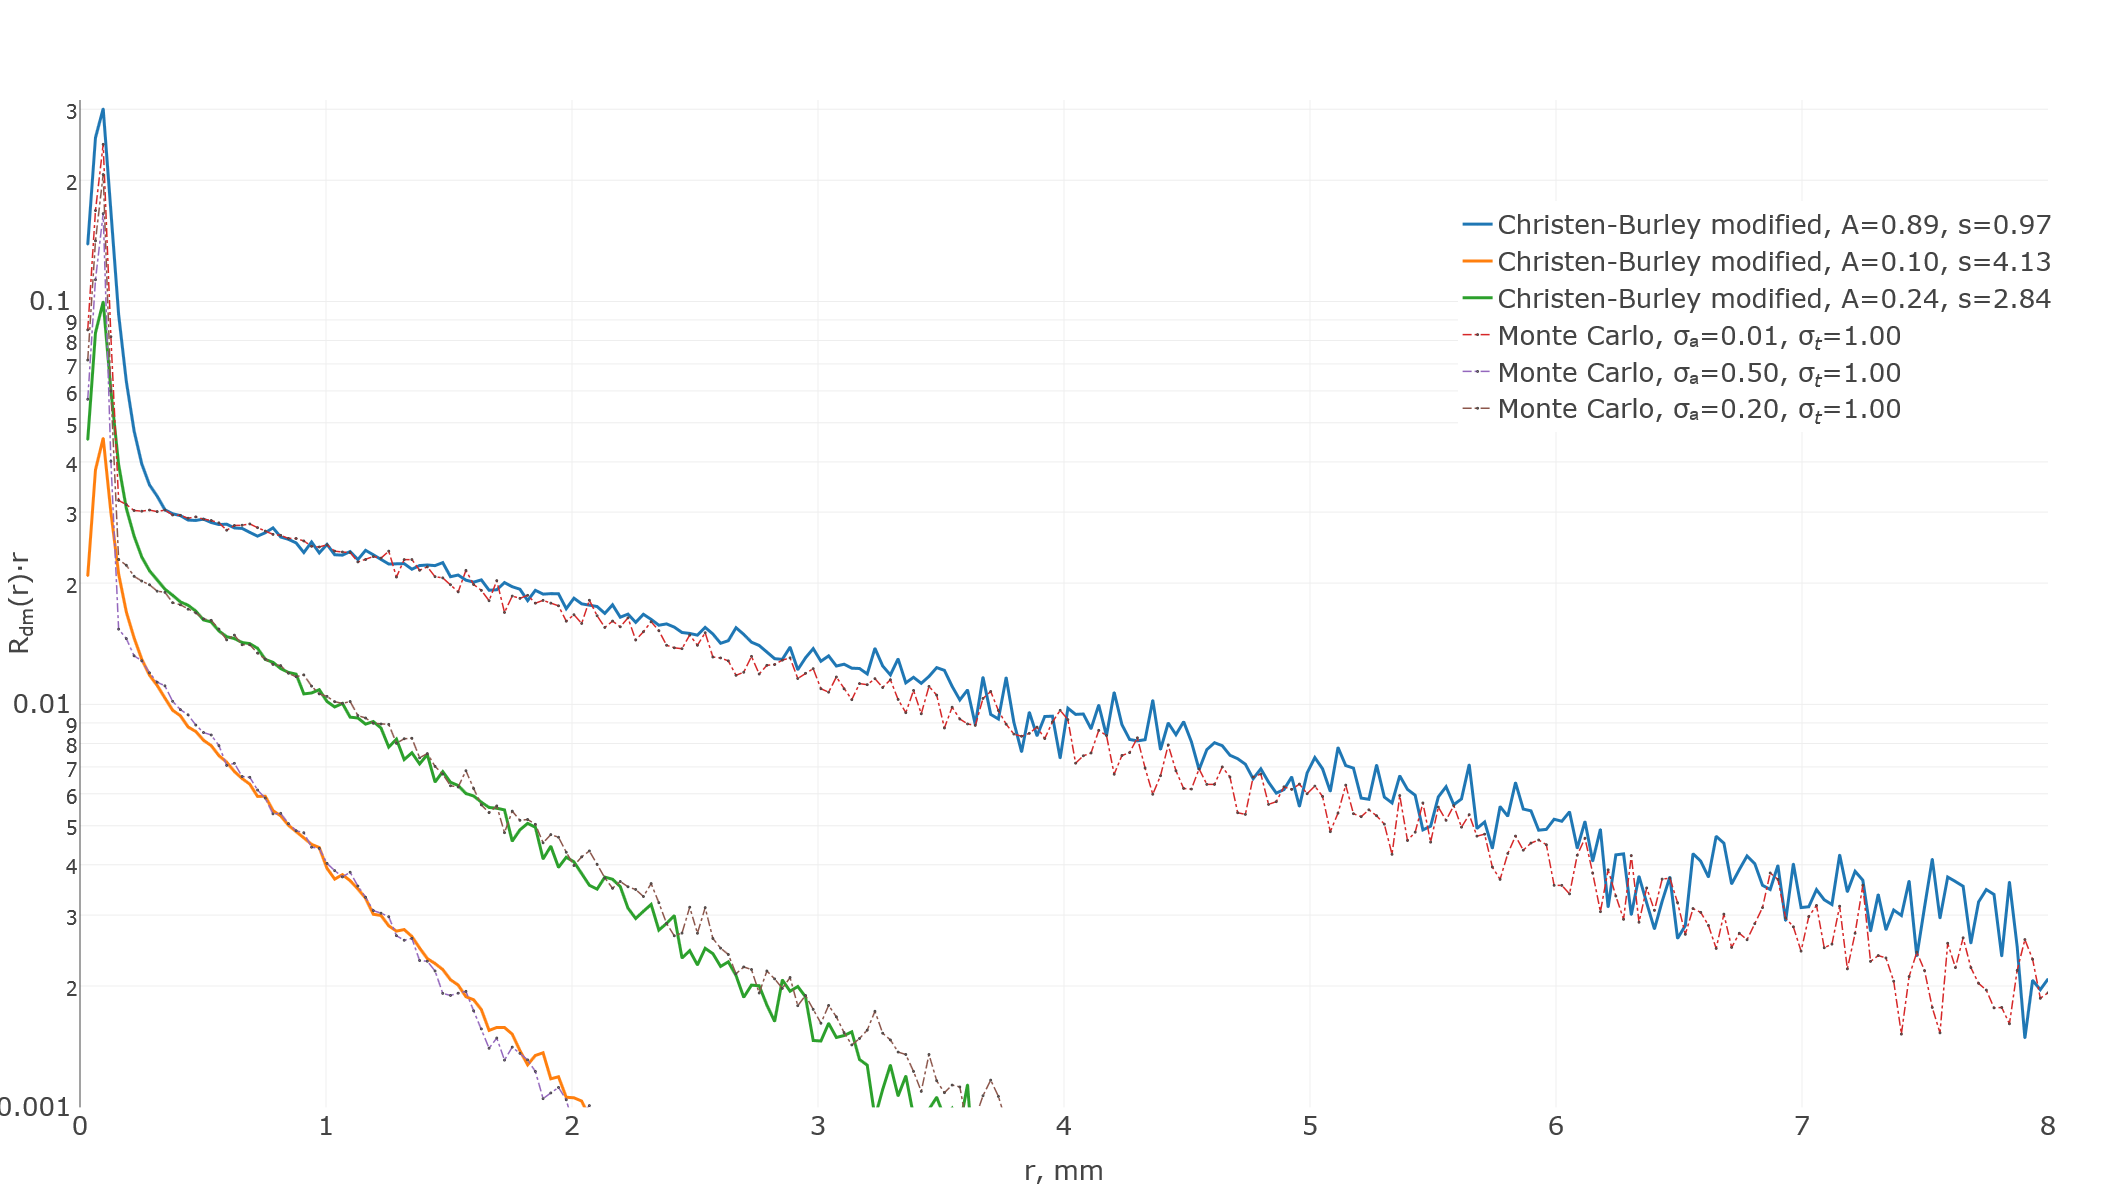
\includegraphics[width=\textwidth]{imgs/plots/cb_modified_fitting}
        \caption{Modified Christensen-Burley over Monte Carlo reference}
    \end{subfigure}

    \caption{Comparison between the original and proposed techniques in log-y
    scale. Monte Carlo references are in thin lines. The parameters $A$ and $s$ of the model are
    computed according to the }
    \label{fig:burley_fitting}
\end{figure}

As we can see from the plots \ref{fig:burley_fitting}, there is a tendency for
the original model to overestimate outgoing radiant exitance in the region close
to the light source. It is also noticeable as a an extra blurriness of the rendered stripe at
\ref{fig:burley_searchlight_renders}. This trend was observed in many experiments with different optical
properties of the material.

The proposed model to improve the Christensen-Burley BSSRDF profile includes the splitting of the
scaling parameter $s$ and using two different factors for each of the exponents:
\begin{equation}
\label{eq:burley_modified}
R_{dm}(r) = A\dfrac{te^{-tr}+se^{-sr/3}}{8\pi r}
\end{equation}

This modification allows to control the weight the exponents independent of each other and adjust
the profile to better match the corresponding Monte Carlo reference. The particular form of $s$ and
$t$ is based on the original function developed by Burley and Christensen. The coefficient $s$ of
the proposed model has the same form as the original equation (\ref{eq:cb_scaling}). But the form of
$t$ is adjusted with the multiplication of the linear function:
\begin{equation}
\label{eq:cb_scaling_modified}
t=s*(20A+2)=(1.85-A + 7|A - 0.8|^3)*(20A+2)
\end{equation}

The result of such modification and the comparison to the original profile is shown at figures
\ref{fig:burley_fitting} and \ref{fig:burley_searchlight_renders}.

\textit{Note about Monte Carlo references:
There are consistent results achieved for Searchlight experiment
(semi-infinite slab with narrow pencil beam of light pointing from top in the normal
direction). In which brute force Monte-Carlo simulation in P2 (path tracing) was
compared to PTDL approach and also to hybrid technique used in Mitsuba
renderer. All three methods produce the same result in the scope of their
capabilities. It give us some assurance of the correctness of the Monte-Carlo
algorithms which are used as the references.}